\begin{figure}[htbp]
\centering
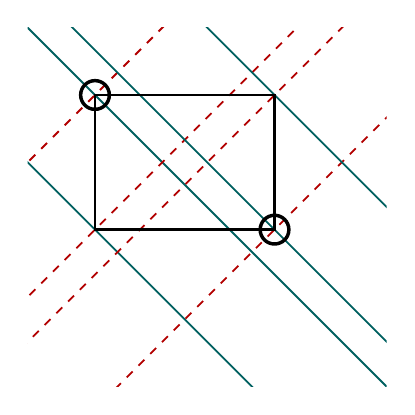
\begin{tikzpicture}[x=.57cm,y=.57cm]
 \bcuadricula{8}
 \begin{scope}
  \clip (0,0) rectangle (8,8);
  \foreach \rr/\cc in {2/2,5/2,5/6,2/6}{
   \draw[teal!75!black,line width=.65pt] ({\cc-.5},{8.5-\rr}) ++(-8,8) -- ++(16,-16);
   \draw[red!70!black,dashed,line width=.65pt] ({\cc-.5},{8.5-\rr}) ++(-8,-8) -- ++(16,16);
  }
 \end{scope}
 \draw[black,line width=1pt] (1.5,6.5) rectangle (5.5,3.5);
 \foreach \rr/\cc in {2/2,5/2,5/6,2/6}{\bmarca{8}{\rr}{\cc}}
 \draw[black,line width=1.25pt] (1.5,6.5) circle[radius=.32];
 \draw[black,line width=1.25pt] (5.5,3.5) circle[radius=.32];
\end{tikzpicture}
\caption{Rectángulo en un tablero vacío de orden ocho. Las filas se numeran desde uno de arriba abajo
y las columnas desde uno de izquierda a derecha. Los vértices en orden son $e_1=(2,2)$, $e_2=(5,2)$,
$e_3=(5,6)$ y $e_4=(2,6)$. Pasan por ellos cuatro diagonales $i-j$ (continuas) y cuatro antidiagonales
$i+j-1$ (discontinuas). Los círculos eligen los vértices opuestos $e_1,e_3$. El término de la
expansión con $T=\{1,3\}$ tiene signo $(-1)^{4-2}=+1$.}\label{fig:rectangulo}
\end{figure}
